\documentclass[main.tex]{subfiles}
\begin{document}
    Le simulazioni mostrano che fissata la città, l'indice di traffico aumenta all'aumentare delle automobili
    e tende a 1 per il numero di automobili che tende a zero. Ovviamente tale simulazione non avrebbe senso, per ciò 
    partiamo da almeno 1 macchina nella città, l'indice di traffico che emerge dalla simulazione con una sola macchina
    sarà 1 poiché non può esistere un rallentamento.
    In Fig. \ref{fig:1} è riportato l'esito di circa 70 simulazioni che incrementano di 1 il numero di automobili da 1 a 2000.
    Ciò è stato fatto su una città $5 \times 5$ senza senzi univi per verificare che effettivamente il traffico aumentasse
    all'aumentare delle auto.
    \begin{figure}[H]
        \centering
        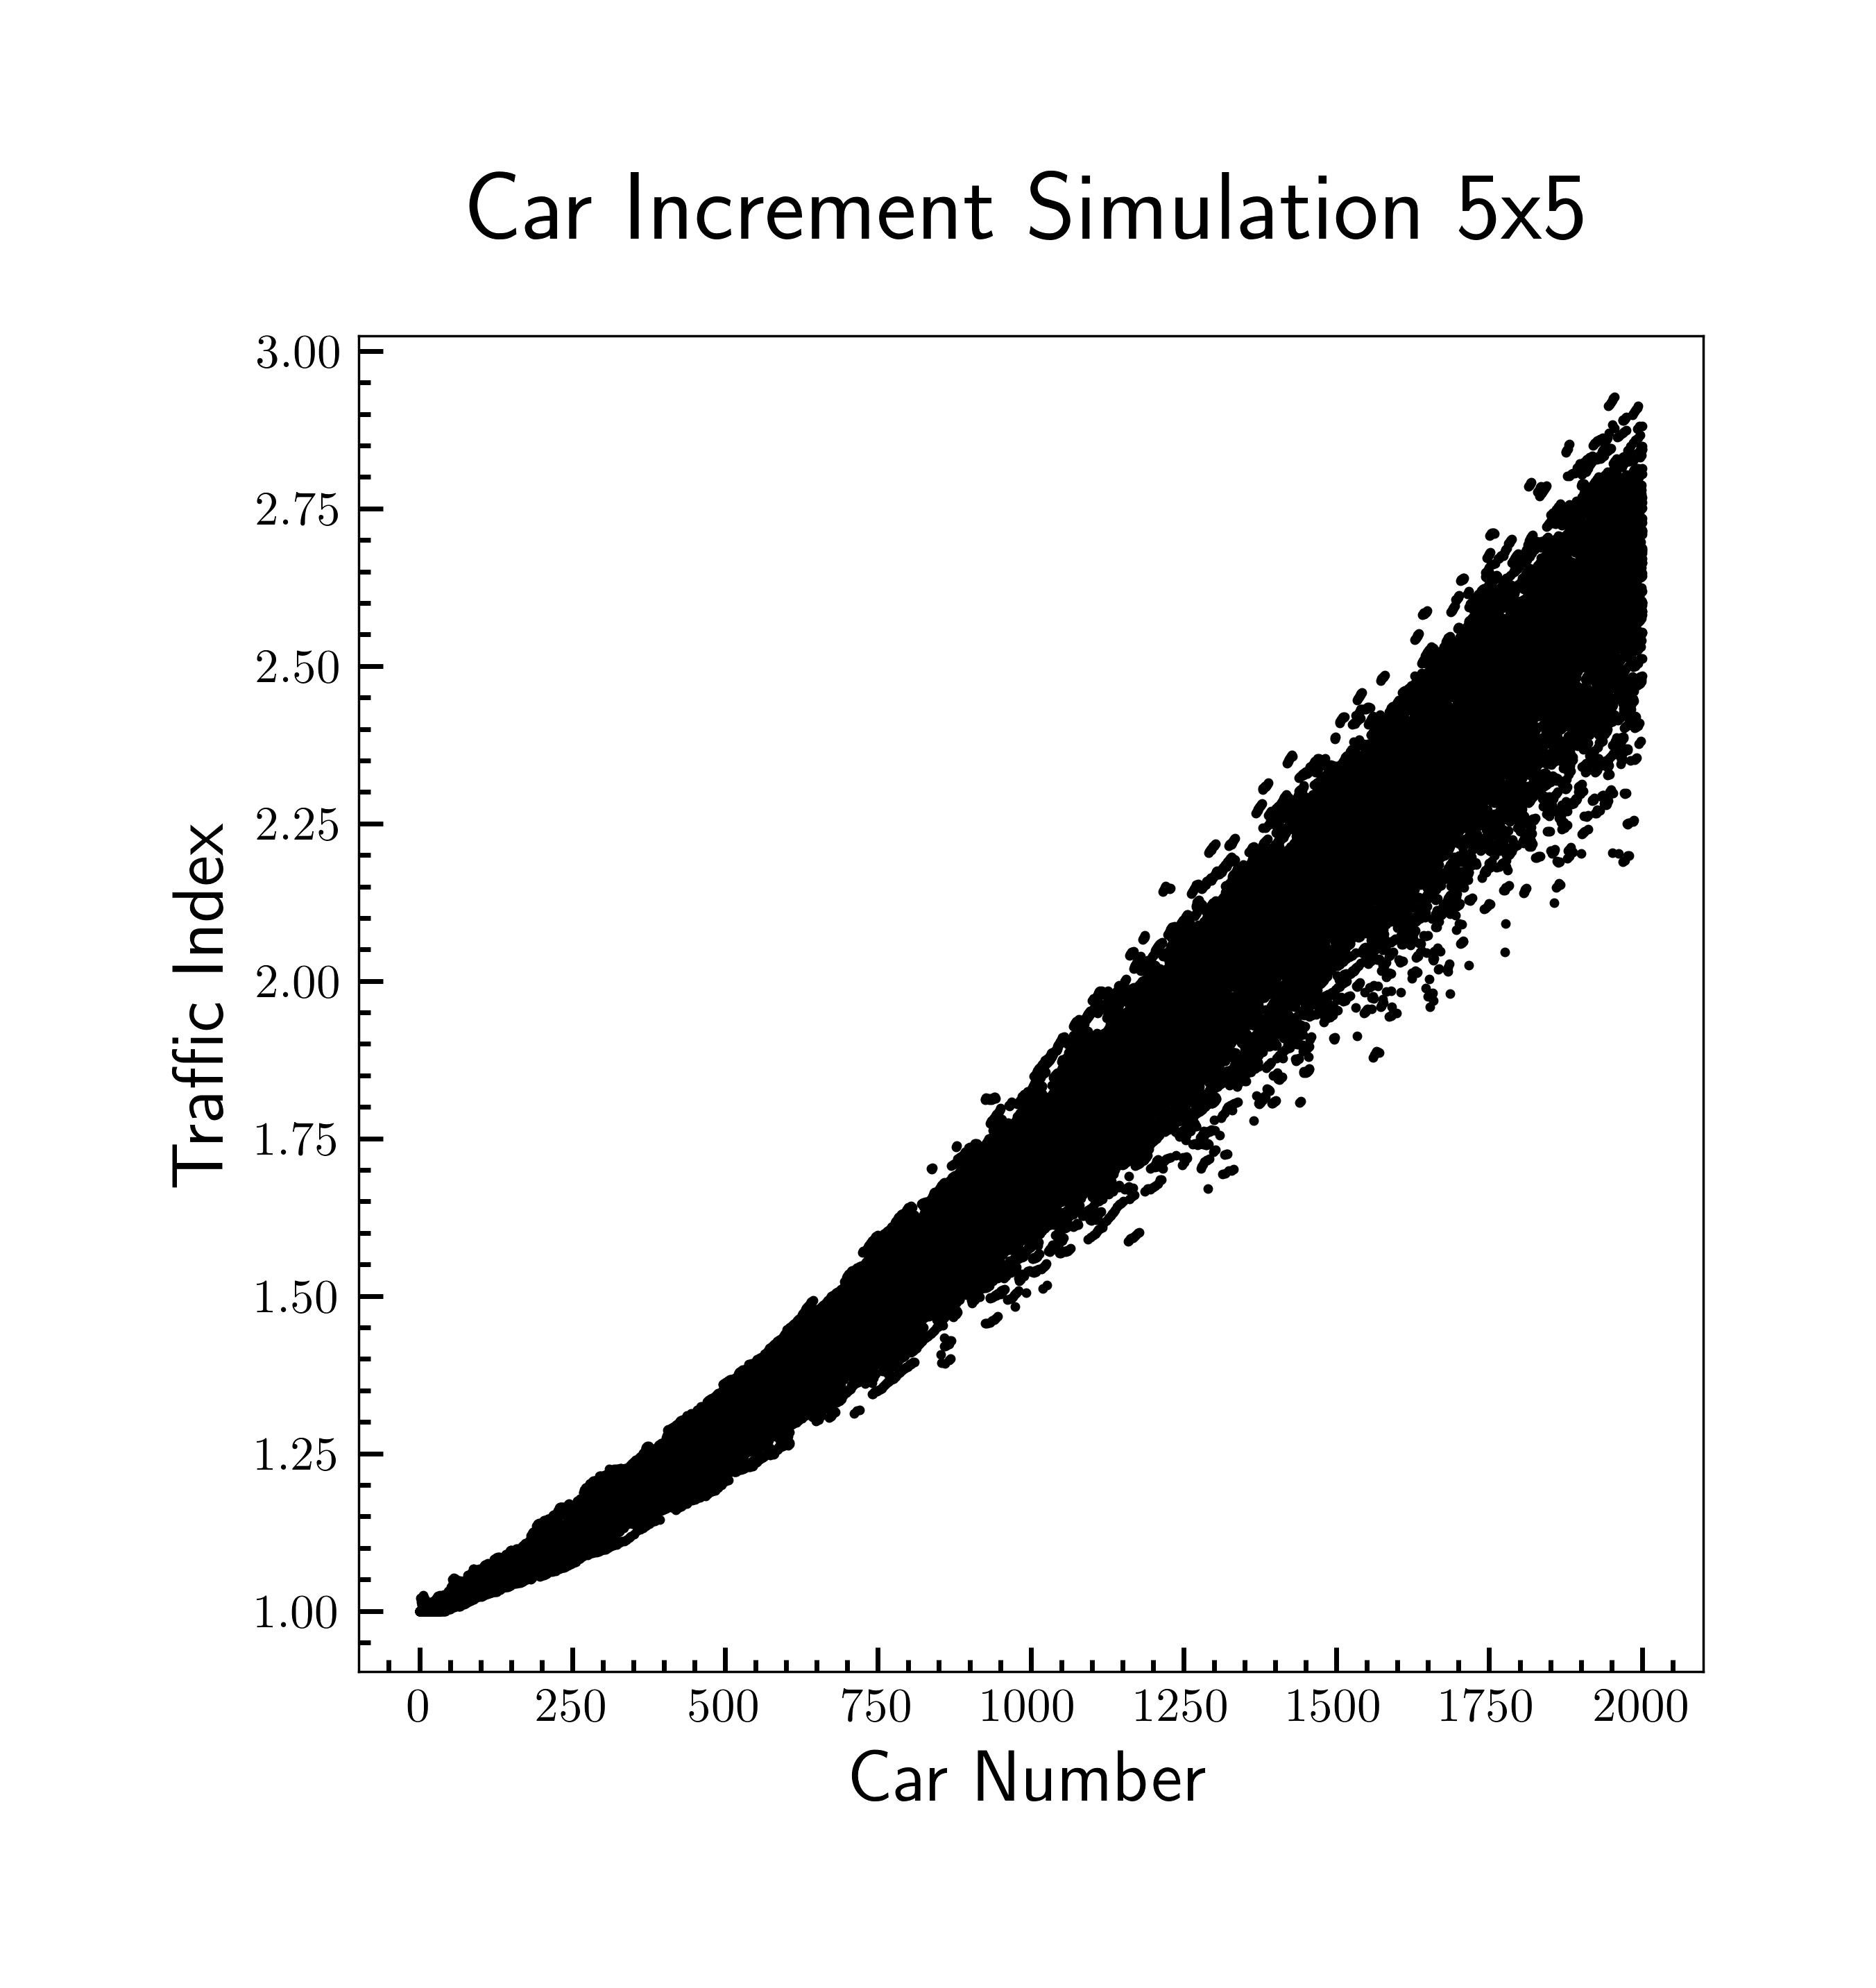
\includegraphics[width=9cm, height=9cm]{car_increment5x5.png}
        \caption{Car Increment Simulation su una città $5 \times 5$ senza sensi unici.}
        \label{fig:1}
    \end{figure}

    \newpage

    In Fig. \ref{fig:2} è invece riportato l'esito di una simile simulazione su una città $7 \times 7$.
    \begin{figure}[H]
        \centering
        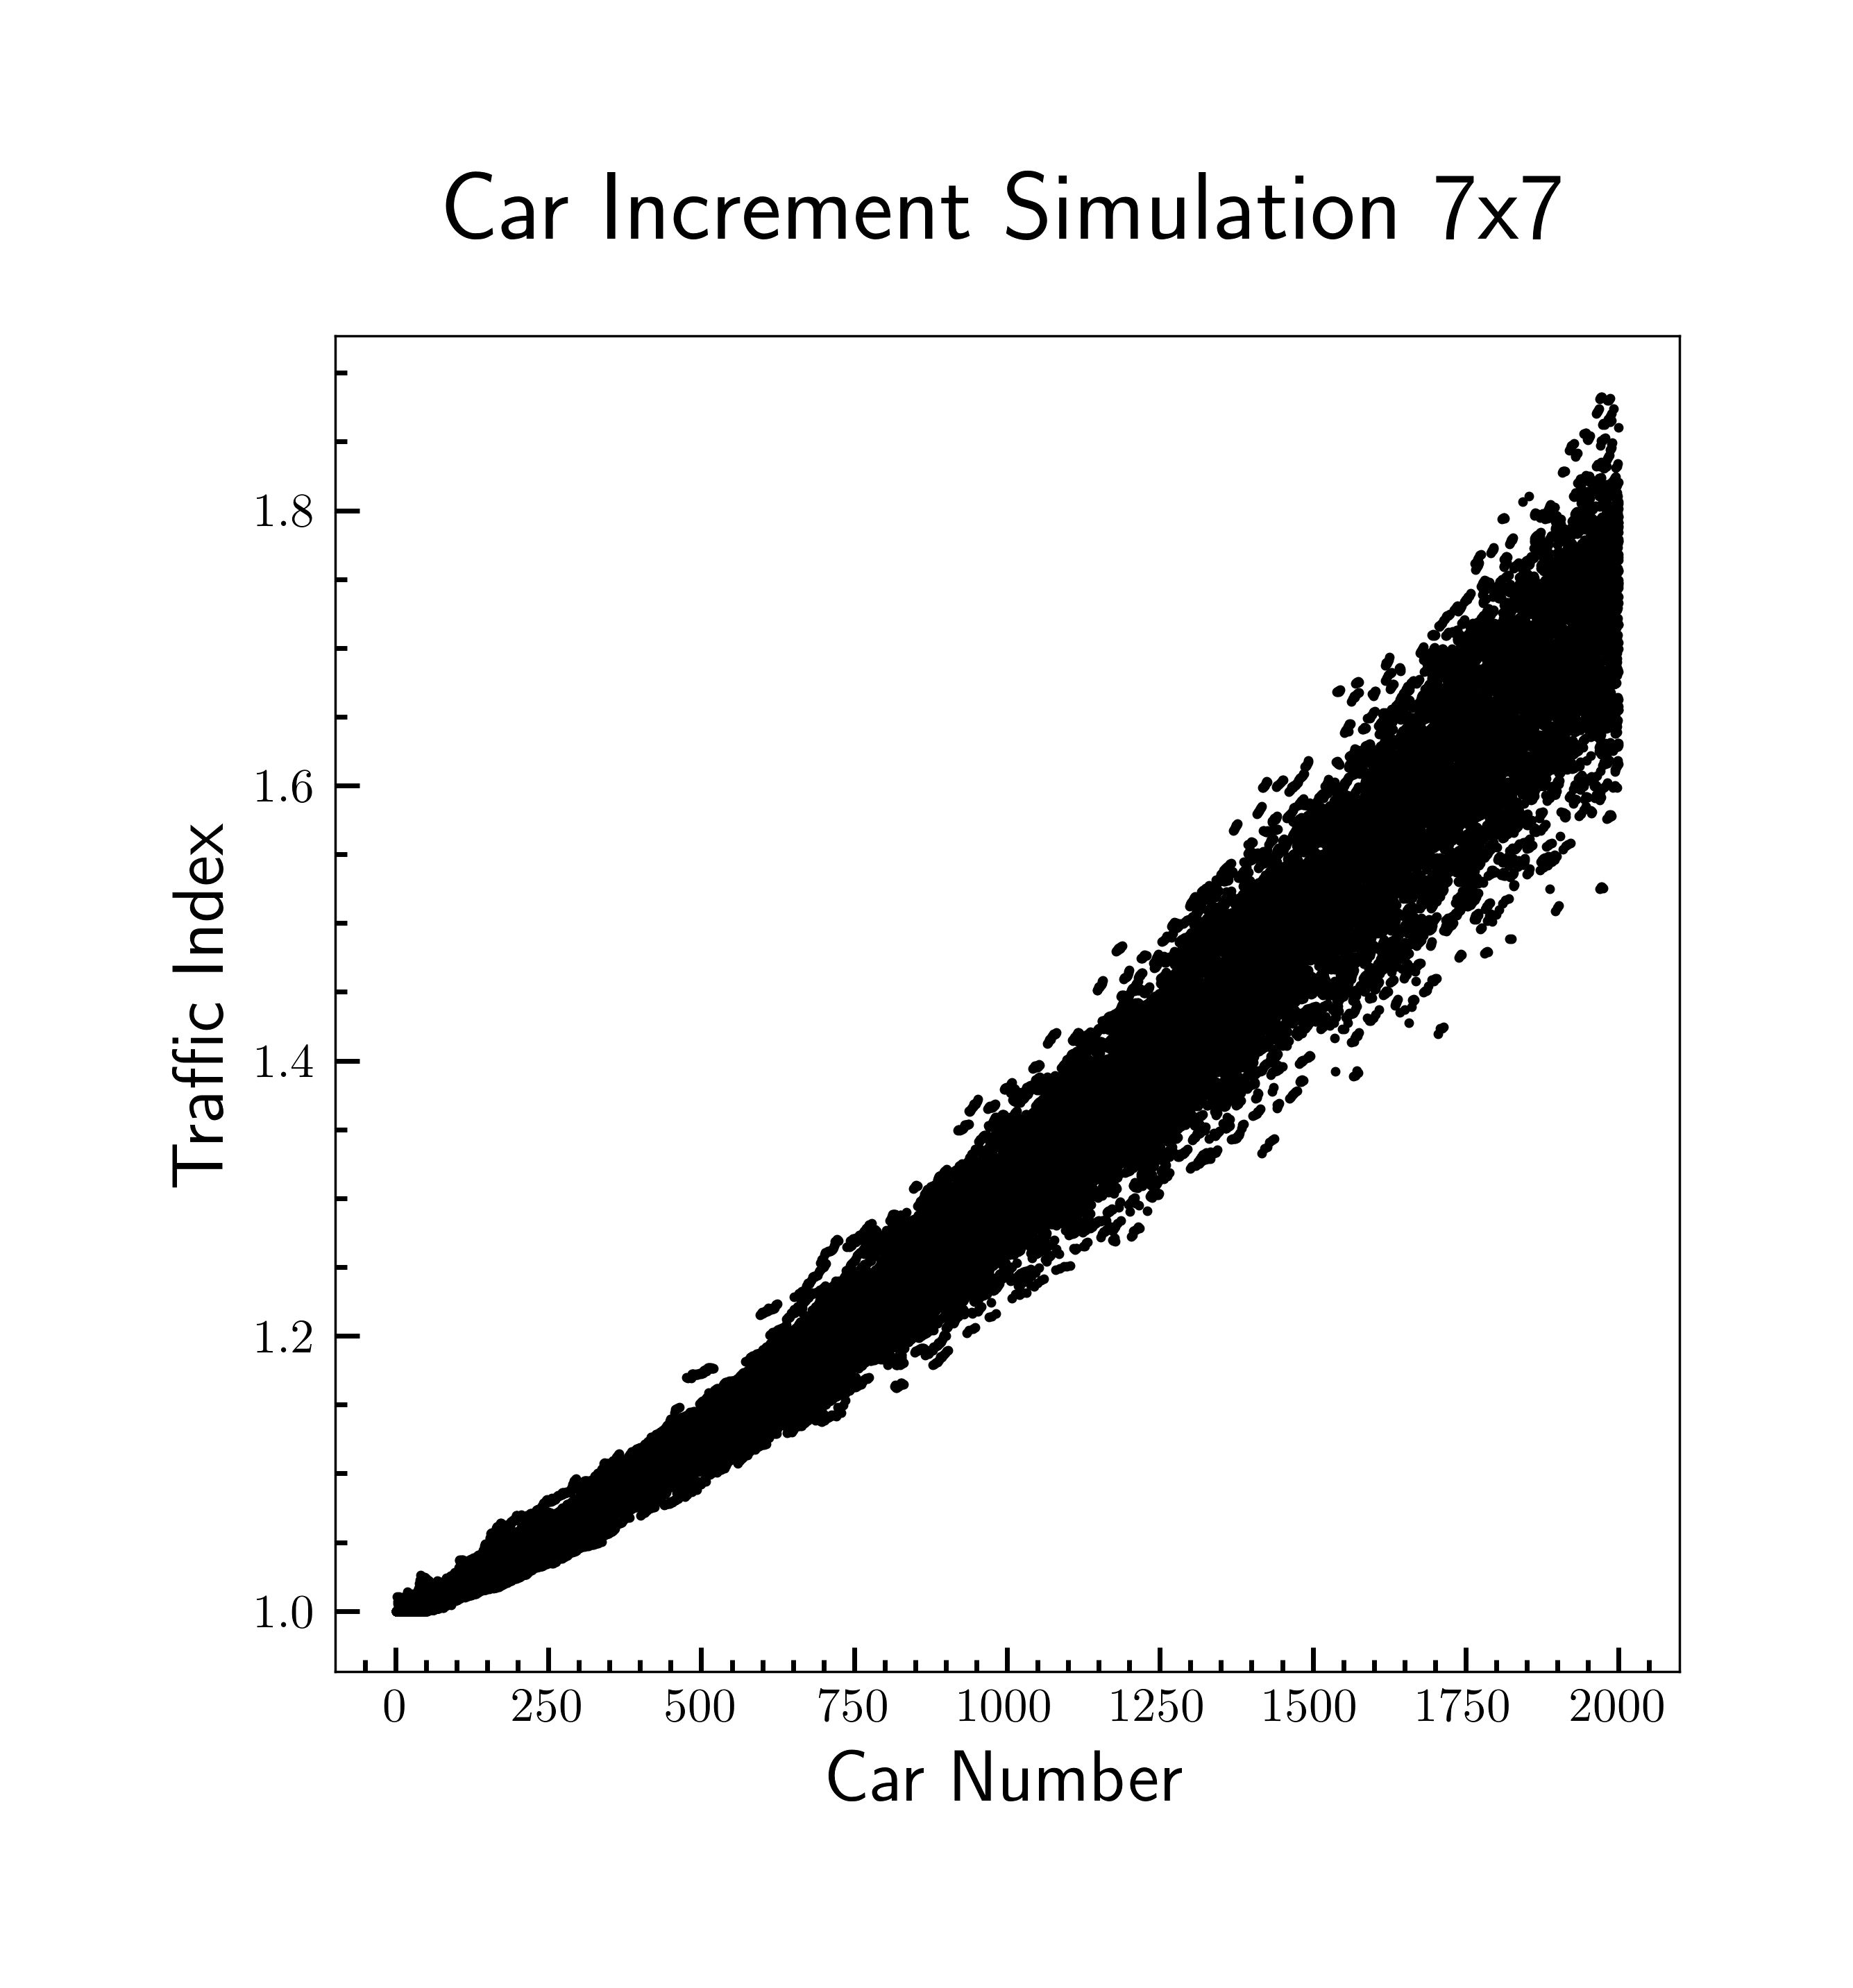
\includegraphics[width=9cm, height=9cm]{car_increment7x7.png}
        \caption{Car Increment Simulation su una città $7 \times 7$ senza sensi unici.}
        \label{fig:2}
    \end{figure}

    Per entrambe queste simulazioni si è usata la seguente statistica delle strade:
    \begin{itemize}
        \item media della lunghezza : 20
        \item deviazione standard della lunghezza : 10
        \item lunghezza massima : 30
        \item lunghezza minima : 10
    \end{itemize}

    Un' osservazione interessante che può essere fatta a partire da queste statistiche è che su città rispettivamente
    $5 \times 5$ e $7 \times 7$ generano una superficie stradale media data da $20 \times 5 \times 4 \times 2 = 800$ e
    $20 \times 7 \times 6 \times 2 = 1680$. Data questa considerazione, notiamo che quando il numero di auto è confrontabile con 
    la superficie media nelle due simulazioni l'indice di traffico si trova sempre attorno a 1.5.
    Perciò possiamo pensare che senza ulteriori modifiche topologiche, l'indice di traffico su una città a griglia
    senza sensi unici dipenda esclusivamente dalla densità di automobili.

    Il fatto che a densità uguale a 1 il programma non si blocchi è dovuto ad un controllo che fa partire le auto con diversi ritardi,
    quindi non tutte le auto indicate da car number saranno nella città contemporaneamente.
    Da questa anilisi preliminare possiamo concludere che il traffico emerge dal nostro modello e dipende dalla densità di auto,
    come suggerito da tutti i modelli di traffico esistenti.

    Per vedere se aumentare il numero di sensi unici è conveniente, abbiamo fatto una simulazione aumentando 

    
\end{document}